\section{Analysis}
\label{Analysis}

\subsection{Cancelation of Detector Efficiencies, Drifts, and Geometric Phase Space}
\label{subsec:SPDPCancelation}
The efficiency and acceptance of the neutron detection system varies greatly over its opening angle range from 20$^{\circ}$ to 180$^{\circ}$, as illustrated in Fig.~\ref{fig:SPDPNormalization}(a).
This is both due to the neutron detection system's non-spherical symmetry and to varying efficiency as a function of particle position on the detector.
In order to give a result that is sensitive to angular correlations but insensitive to detector efficiencies and experimental drifts, angular correlation is always calculated by the following fraction:
\begin{displaymath}
\text{angular correlation }  \propto \frac{nn_{\text{corr}}(\theta)}{nn_{\text{uncorr}}(\theta)},
\end{displaymath}
 where $nn_{\text{uncorr}}(\theta)$\footnote{While this notation implies that coincident events are only due to neutrons, about 3\% of total  $nn_{\text{corr}}(\theta)$ events are not due to neutrons. This was determined by comparing data from a non-neutron producing Al target to that from a $^{238}$U target (see Fig.~\ref{fig:Noise})} is produced from a manufactured set of opening angles, hereafter denoted by $nn_{\scaleto{DP}{4pt}}(\theta)$, by pairing neutron events that occurred during different pulses, and $nn_{\text{corr}}(\theta)$ is the accidental subtracted opening angle distribution, which is described in section~\ref{Reconstruction of Accidental Coincidence}.

$nn_{\scaleto{DP}{4pt}}(\theta)$ is constructed by examining pulses in pairs of two, which are required to have occurred within 0.2 seconds of each other, and for those pairs that have an event in both pulses, the opening angle is calculated between the events in the same way that it would be for coincident events from the same pulse.
$nn_{\text{uncorr}}(\theta)$ is a subset of $nn_{\scaleto{DP}{4pt}}(\theta)$ which only uses pulse pairs that have two neutron events in both pulses, and, as a result, four pairs of uncorrelated neutrons can be formed from each pulse pair used in $nn_{\text{uncorr}}$. 
The reason for doing this is to increase the percentage of pairs of fission neutrons in $nn_{\text{uncorr}}(\theta)$, as opposed to pairs of neutrons from $(\gamma,n)$.
This is an important point because the detection of multiple neutrons from $(\gamma,n)$ are completely removed from $nn_{\text{corr}}(\theta)$ (the numerator in $\frac{nn_{\text{corr}}(\theta)}{nn_{\text{uncorr}}(\theta)}$) due to the subtraction of accidental coincidences.

As long as the numerator and denominator are comprised of neutron pairs with the same energies, the ratio between $nn_{\text{corr}}(\theta)$ and $nn_{\text{uncorr}}$ does not depend on detector efficiency.
Thus, because the two energy distributions are not necessarily the same, the following calculation gives a result that is integrated over some set, $\C$, of neutron-neutron energies (also referred to as an \emph{energy cut}):
\begin{equation}
\label{eq:I_results}
\text{integrated angular correlation }\propto  \iint \limits_{(E_1,E_2 ) \in \C}  \frac{nn_{\text{corr}}(\theta_{nn}, E_1, E_2)}{nn_{\text{uncorr}}(\theta_{nn},E_1, E_2)} dE_1 dE_2
\end{equation}
Because Eq.~\ref{eq:I_results} exhibits no dependance on experimental parameters, the same quantity can be calculated from the output of a model such as FREYA and compared by side-by-side with measurements.

Figure~\ref{fig:SPDPNormalization}(a) shows the measured $nn_{\text{corr}}(\theta)$ yield distribution of neutrons from the photofission of $^{238}$U.
The structure seen here is reflective of the underlying two-neutron angular correlations as well as the geometric acceptance and efficiencies of the neutron detectors.
Figure~\ref{fig:SPDPNormalization}(b) reveals how a clear picture of two-neutron correlations emerges when taking the ratio between $nn_{\text{corr}}(\theta)$ and $nn_{\text{uncorr}}(\theta)$.

The photo-disintegration of D$_{2}$O, which produces uncorrelated neutrons, gives a flat distribution in cos$(\theta_{nn})$, as expected (see Fig.~\ref{fig:D2Otheta_nn}).
\begin{figure}[]
\centering
    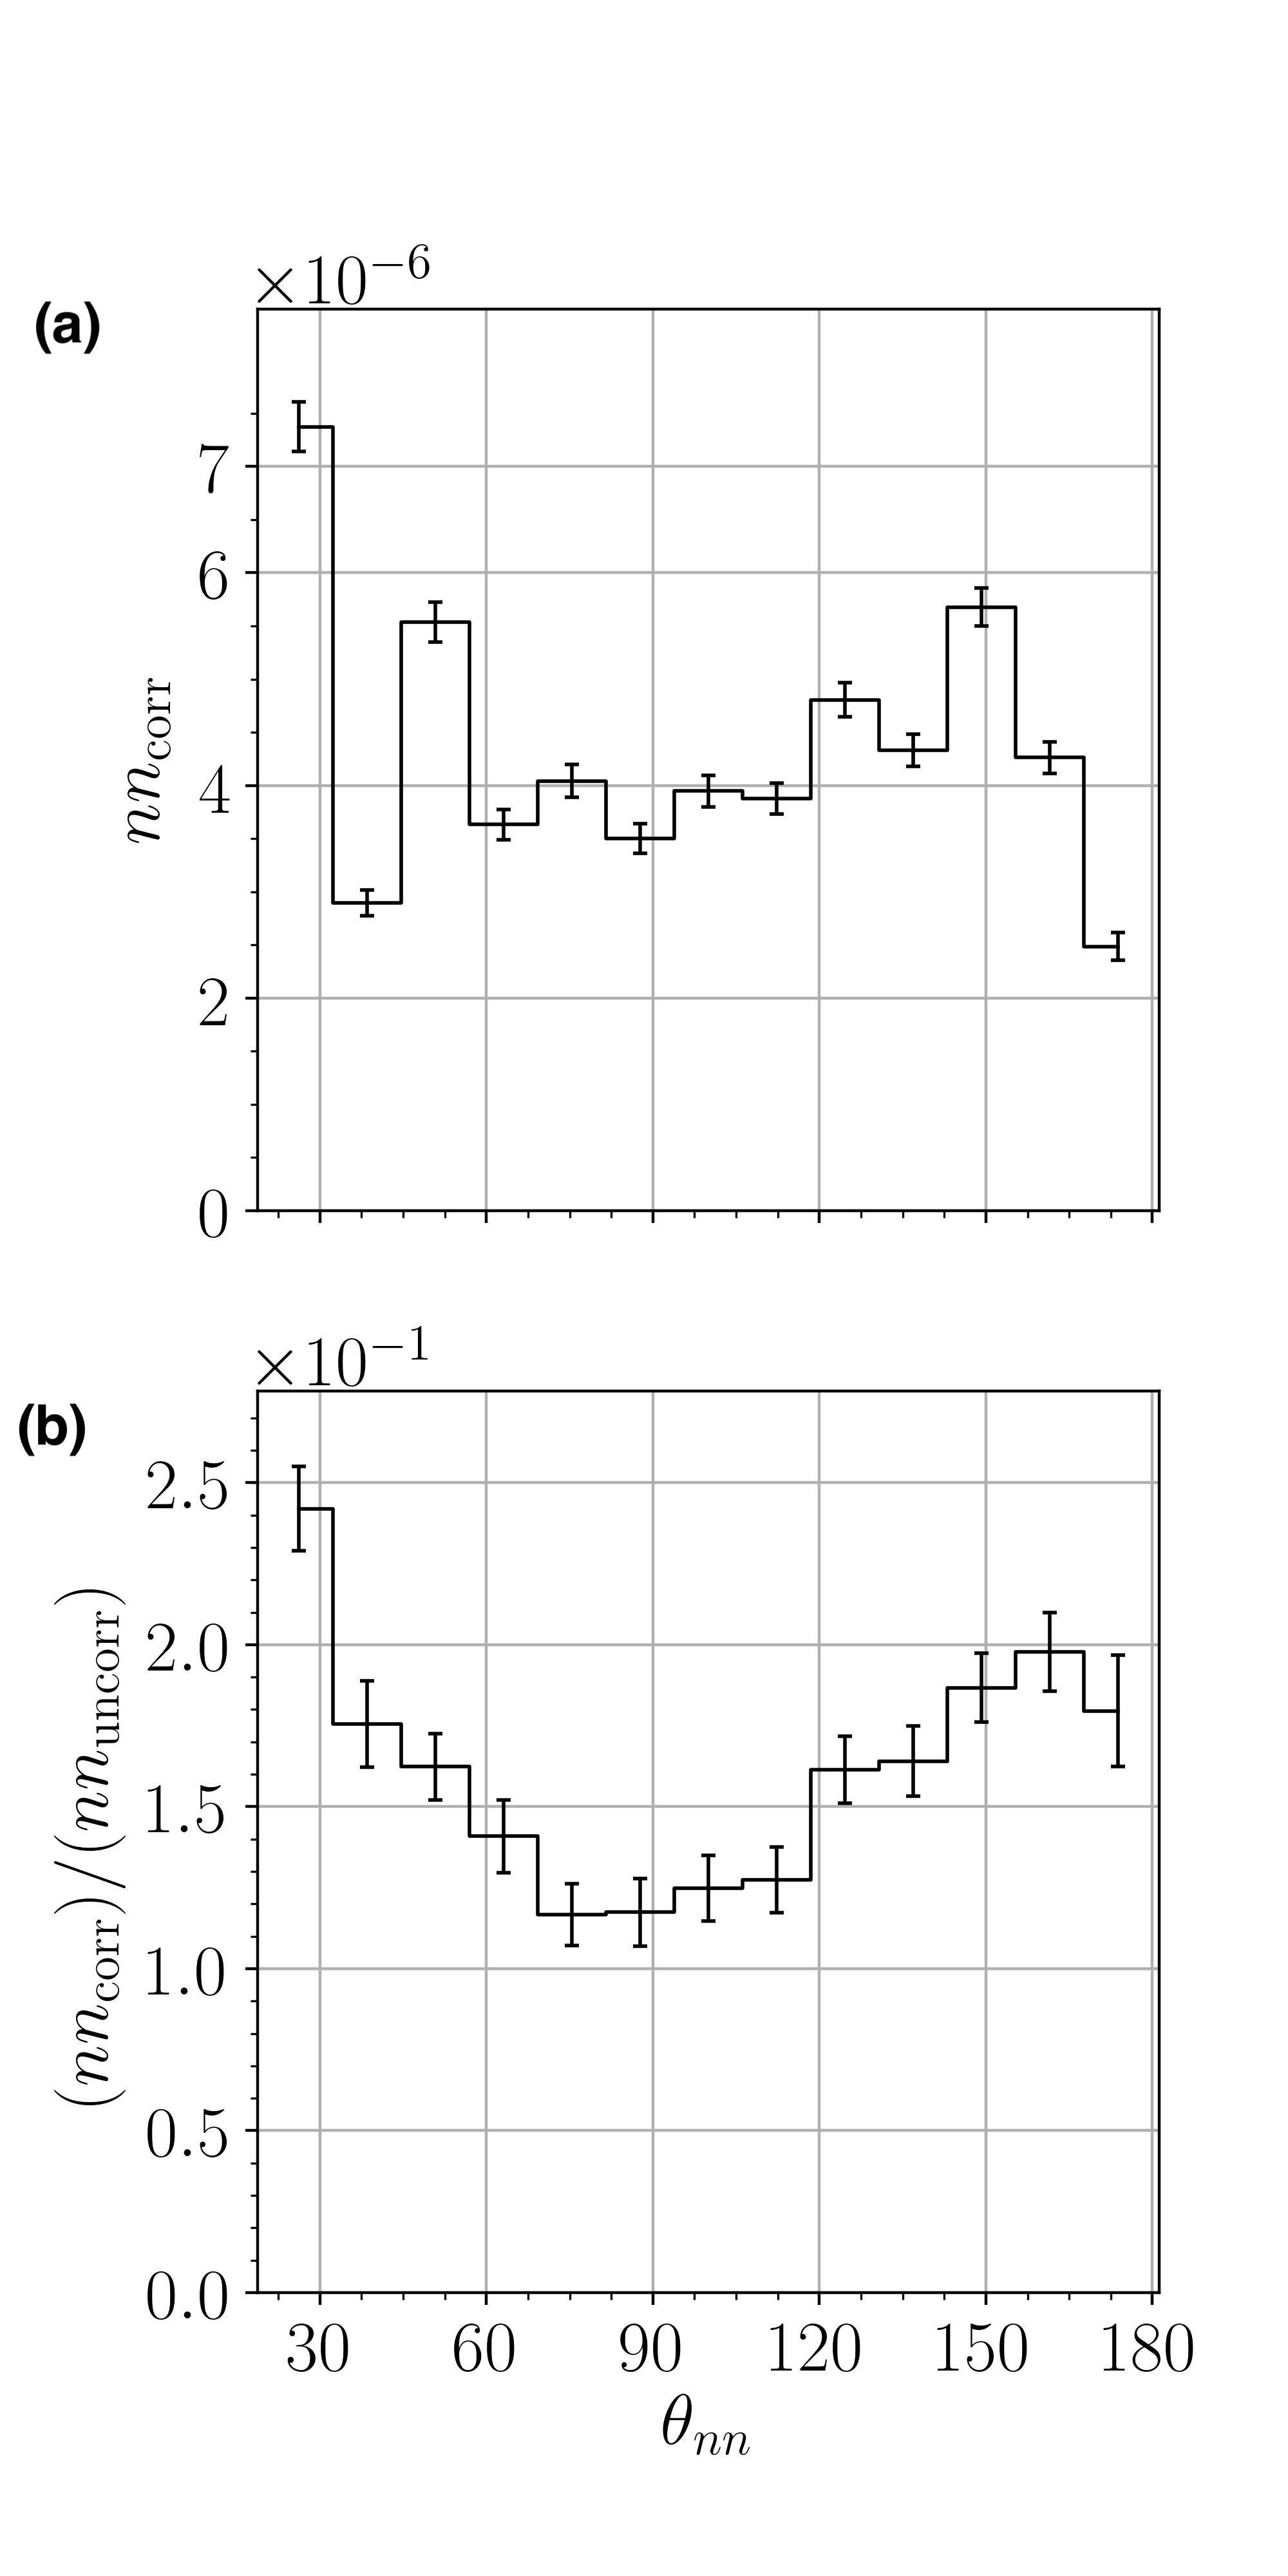
\includegraphics[width=0.7\textwidth]{Content/Methods/SPDPNormalization.png}
    \caption{(a) Two-neutron opening angle distribution from the photofission of $^{238}$U before normalization, and, (b) after normalizing to the distribution of uncorrelated two-neutron events from different pulses.
    All measured neutrons have an energy greater than 0.4 MeV.}
    \label{fig:SPDPNormalization}
\end{figure}
\begin{figure}[h]
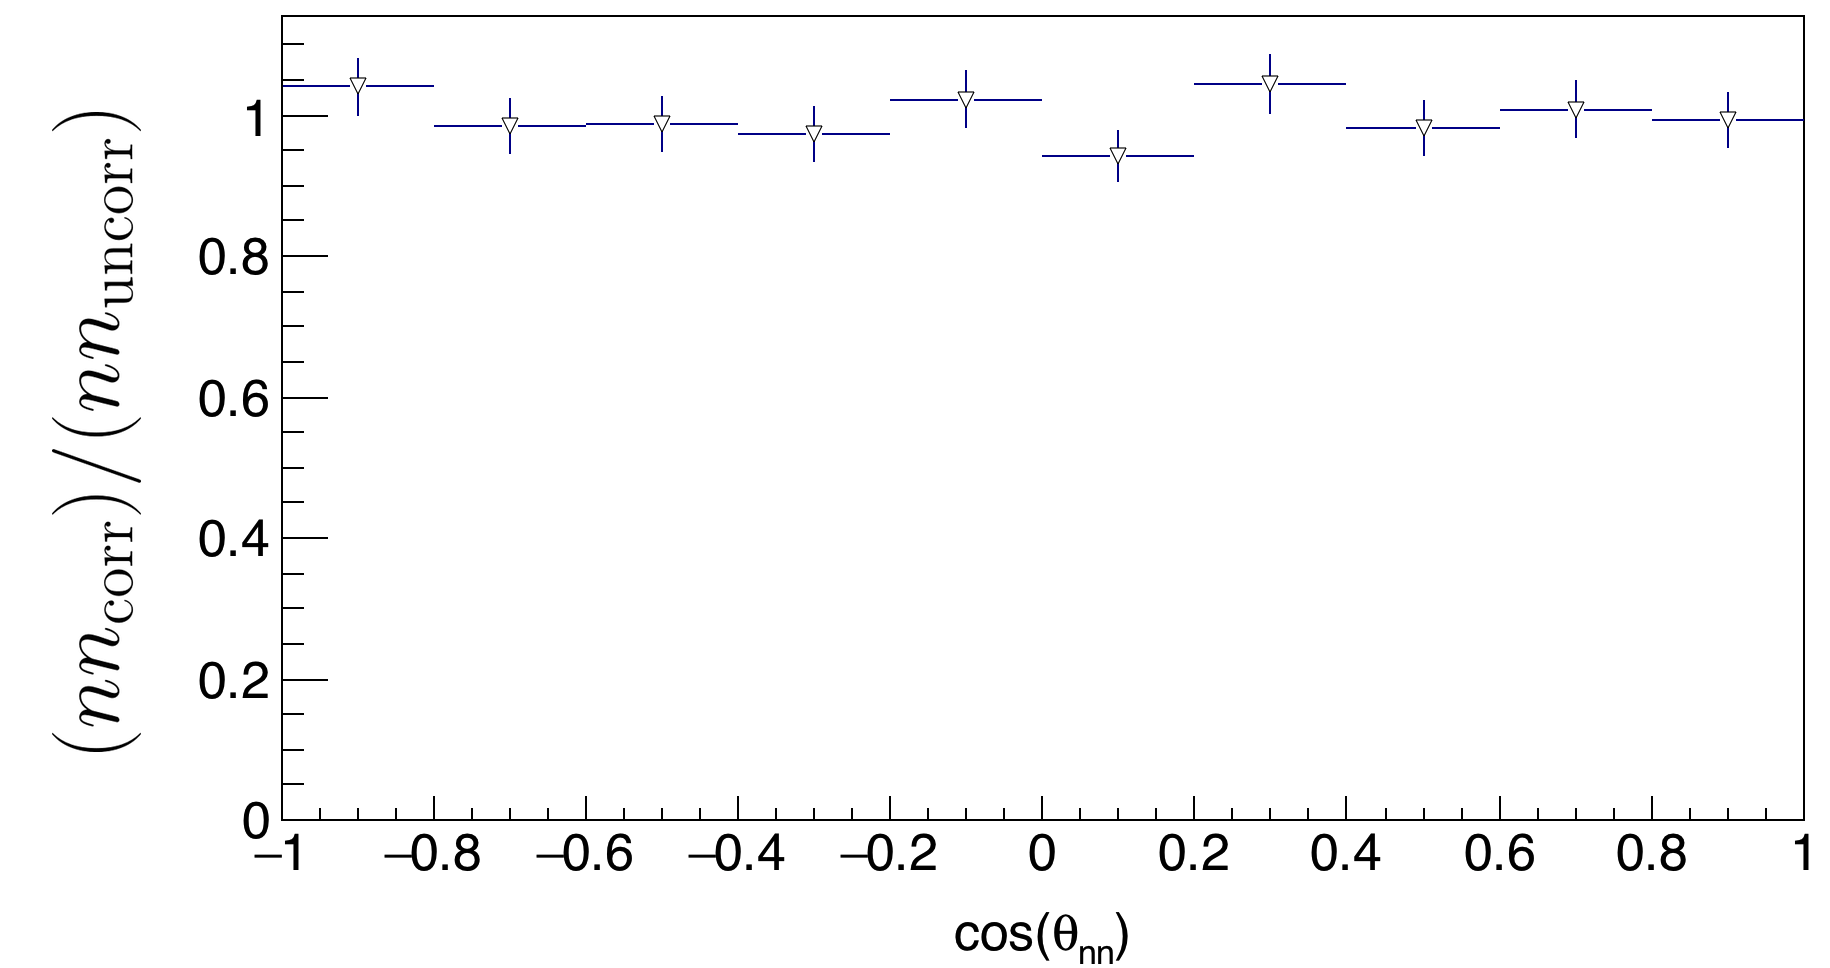
\includegraphics[width=0.9\textwidth]{Content/Methods/D2Otheta_nn.png}
\caption{The opening angle distribution of neutrons from the photo-disintegration of D$_{2}$O  is uniform in cos$(\theta)$, or in otherwise isotropic, as expected.
nn$_{SP}$ and nn$_{DP}$ are the relative yields of neutron formed from the neutron events from the same pulse and from different pulses, respectively.
Here, nn$_{SP}$ arises solely from accidentals.}
\label{fig:D2Otheta_nn}
\end{figure}

\FloatBarrier
\subsection{Subtraction of Accidental Coincidences}
\label{Reconstruction of Accidental Coincidence}
The detection of two uncorrelated events in coincidence, whether caused by neutrons, photons, or noise, is referred to as an \emph{accidental}.
A small number of accidental photon events will exist in the neutron time of flight range because of the smearing of the photon peak.
These events are accidentals, because they are extremely likely to be due to photons from the beam, and not photons from fission.
There are also accidentals due to noise, which can be estimated with a non-neutron producing target made from aluminum (see Fig.~\ref{fig:Noise}).
The accelerator's current was adjusted so that there are, on average, less than 1.0 fissions per accelerator pulse, but nevertheless statistical fluctuations in the number of fissions per pulse result in accidental coincident neutrons that originated from different, and therefore, uncorrelated fissions.
There are also uncorrelated neutrons produced when multiple $(\gamma, n)$ reactions occur in a single pulse.
The $^{238}$U cross-section of $(\gamma, n)$, integrated over the relevant bremsstrahlung energy distribution, is about a factor of 5.5 times greater than it is for photofission (see Fig.~\ref{fig:CrossSection}).
As a result, it is unavoidable that there be a significant number of neutron coincidences caused by multiple $(\gamma, n)$ reactions relative to those caused by correlated fission neutrons.
If not subtracted from the result, the opening angle distribution of uncorrelated neutrons will wash out the signal from correlated neutrons. 
\begin{figure}[]
\centering
    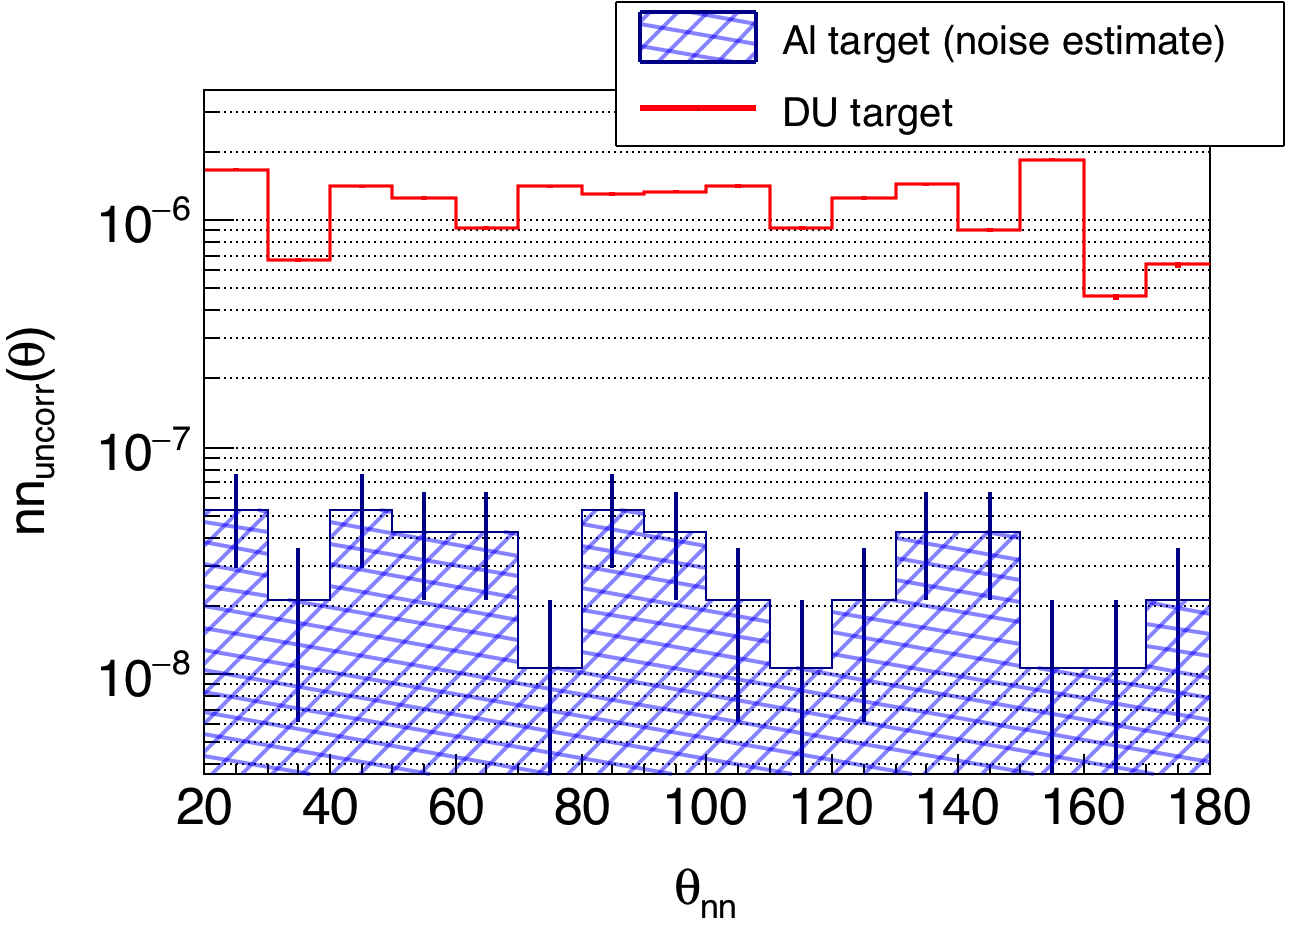
\includegraphics[width=0.8\textwidth]{Content/Methods/Noise.png}
    \caption{An Al target was designed to scatter the same number of photons as the DU target, thus serving as an equivalent non-neutron producing target well-suited to estimate noise.
    The rate of coincident events for the Al target is 3\% that of the DU target. 
        }
    \label{fig:Noise}
\end{figure}
\begin{figure}[]
\centering
    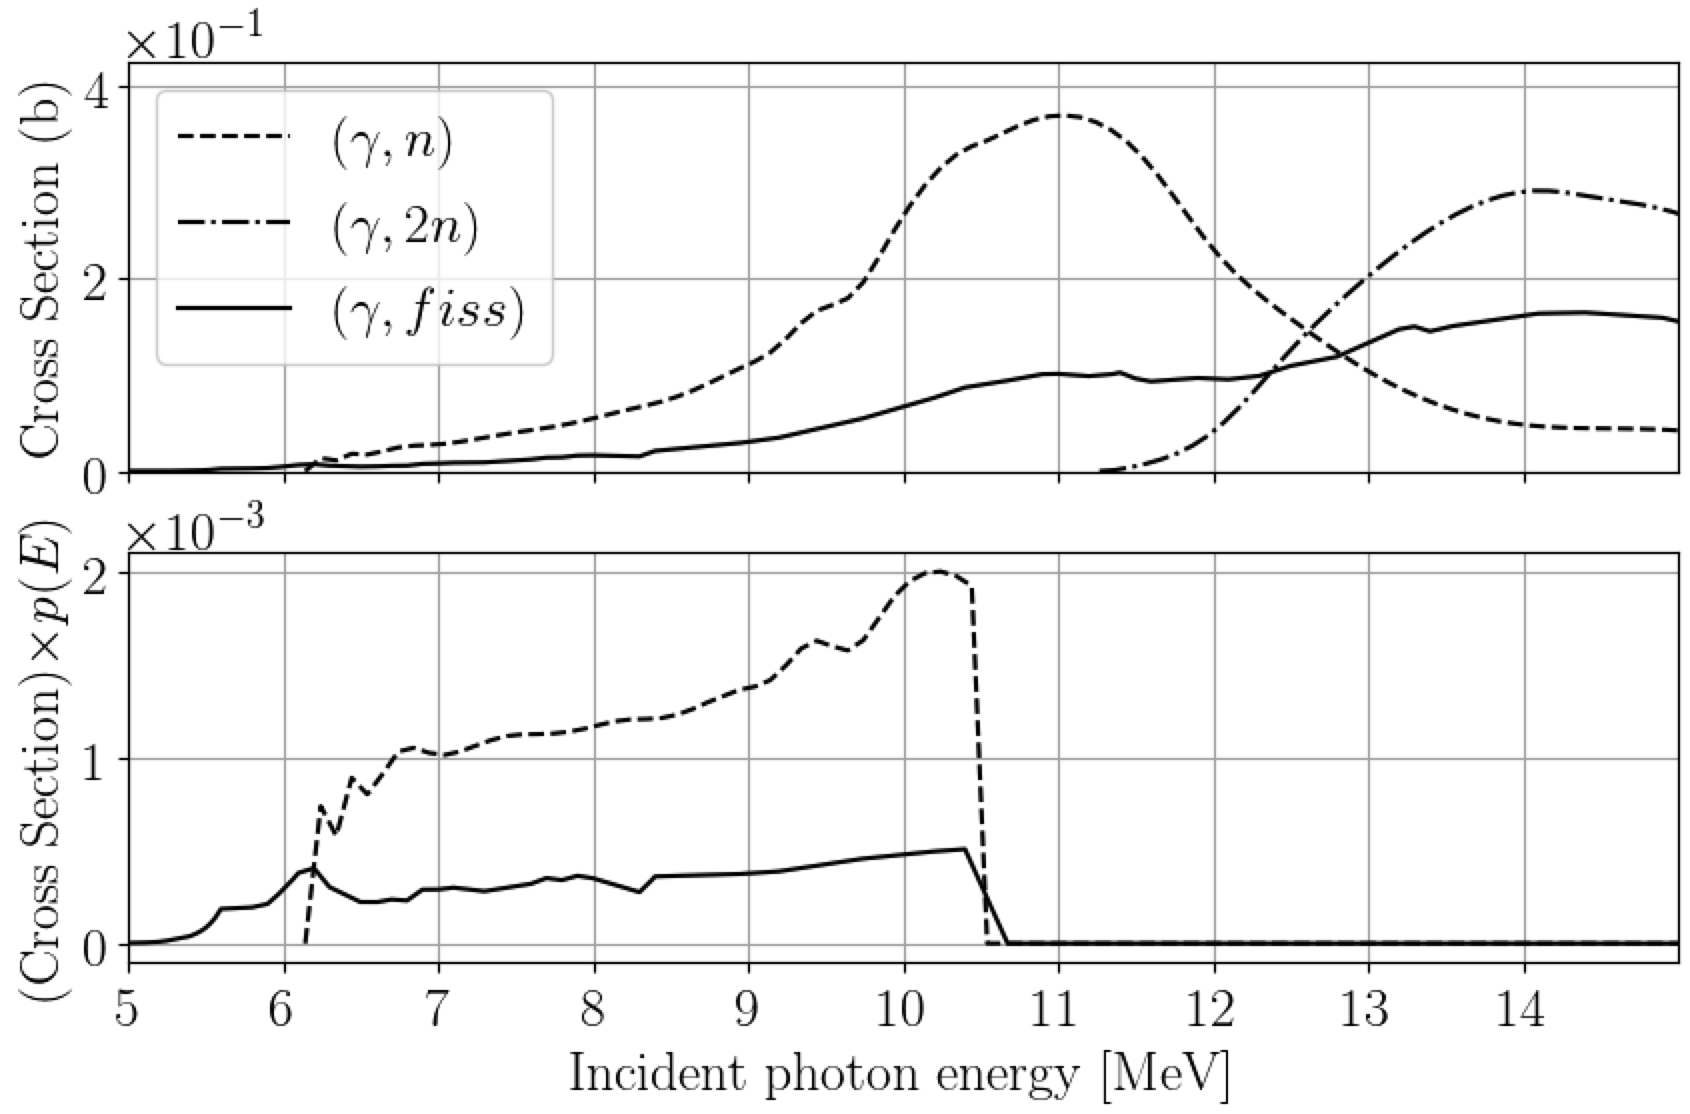
\includegraphics[width=0.95\textwidth]{Content/Methods/CrossSections.png}
    \caption{(top) ENDF cross-sections of $(\gamma$,fiss) and direct $(\gamma$,n) and direct $(\gamma$,2n).
    (bottom) Cross-sections integrated over the simulated relative rate of bremsstrahlung photons that reach the target as a function of photon energy. The integrated cross-sections of $(\gamma, n)$ is 5.5 times greater than for $(\gamma, \text{fiss})$. }
    \label{fig:CrossSection}
\end{figure}
\begin{figure}[]
\centering
    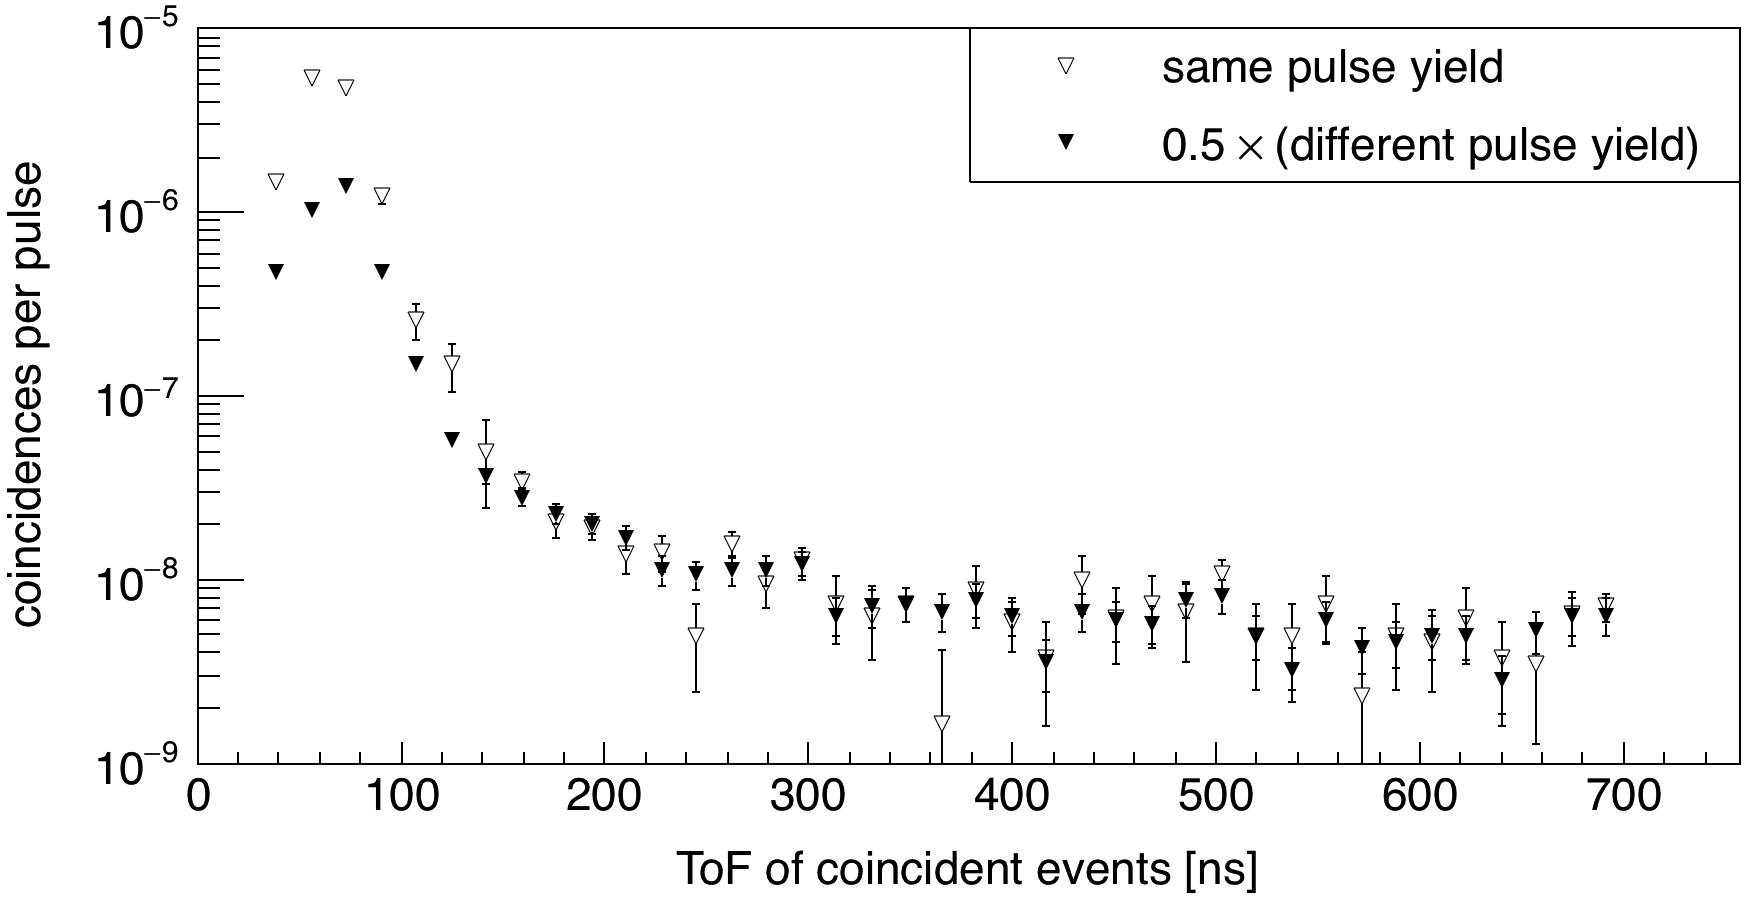
\includegraphics[width=0.9\textwidth]{Content/Methods/NoiseSubtraction.png}
    \caption{The different pulse yield captures the effects of noise due to accidentals.
    The y-axis represents the number of coincidences in which both events had a ToF within a given 20~ns wide bin.
    Because events with a ToF above 120~ns are predominately due to noise, which correspond to a 0.5 MeV neutron, the same pulse yield is equal to 1/2 times the different pulse yield.
    }
    \label{noise_siubtraction}
\end{figure}

The raw measurement consists of a mix of correlated and accidental neutron coincidences, that is
\begin{equation}
\label{eq:corr_uncorr}
nn_{\text{raw}}(\theta)= nn_{\text{corr}}(\theta) + nn_{\text{acc}}(\theta) \,
\end{equation}
where $nn_{\text{raw}}(\theta)$ and $nn_{\text{acc}}(\theta)$ are the rates, per pulse, of the detection of neutron pairs with opening angle of $\theta$ for all events and for accidental coincident events, respectively.

Because accidental coincidences consist of two independent events, it does not matter whether the two events occurred during the same pulse or during two different pulses, given that the two different pulses occurred at around the same time and thus under the same experimental conditions.
Thus, $nn_{\scaleto{DP}{4pt}}(\theta)$ is proportional to $nn_{\text{acc}}(\theta)$.
In other words,  $nn_{\scaleto{DP}{4pt}}(\theta)$ and $nn_{\text{acc}}(\theta)$ have opening angle distributions with the same shape.
However, $nn_{\text{acc}}(\theta)$ is not equal to $nn_{\scaleto{DP}{4pt}}(\theta)$, because there are, on average, twice as many events in a pulse-pair than there are in a single pulse.
For this reason, as the following analysis shows,~$nn_{\text{acc}}(\theta) = \frac{1}{2}nn_{\scaleto{DP}{4pt}}(\theta)$.

The number of uncorrelated events detected per pulse is assumed to follow the poissonian distribution, which describes the occurrence of independent random events.
Let $\lambda$ represent the mean number of uncorrelated events per pulse.
To determine the value of $\lambda$, one needs to know whether a given coincident event is in fact an accidental, as $\lambda$ only quantifies the rate of accidental coincidences.
Such information is not known, but the largest possible value for $\lambda$ is the mean number of events per pulse, because this assumes all events are uncorrelated.
This places an upper bound on $\lambda$ of $3\times 10^{-6}$ for this work, which is small enough to neglect all terms on the order of $\lambda^3$ or greater.

The per-pulse accidental coincidence rate of individual pulses summed over all opening angle bins, denoted by $\sum_{\theta} nn_{\text{acc}}(\theta)$, is equal to the poissonian probability of there being exactly two events detected in a single pulse\footnote{For the sake of brevity, cases of greater than two-fold coincidence are not considered in this analysis, and it is not necessary because of the low detection rates during this work.
It can be shown, however, that accounting for any number of coincidences, from zero all the way up to $\infty$-fold coincident events in a pulse or pulse-pair, will give the same answer.}:
\begin{equation} \label{math:SP}
    \begin{split}
    \sum_{\theta} nn_{\text{acc}}(\theta) & = \frac{e^{-\lambda}\lambda^{2}}{2!} \\
        &\approx \frac{\lambda^2}{{2}} + \mathcal{O}(\lambda^3) \, .
    \end{split}
\end{equation}
For the case of different-pulse pairs, a ``coincidence'' occurs when there is an event in both pulses.
Cases in which there are more than two events can be neglected due to their rare occurrence in this work.
Therefore, the per-pulse rate for different-pulse pairs, again summed over all opening angle bins, is the square of the poissonian probability of there being one event:
\begin{equation} \label{math:DP}
    \begin{split}
   \sum_{\theta} nn_{\scaleto{DP}{4pt}}(\theta)&= \left(e^{-\lambda}\lambda\right)^{2} \\
    &\approx \lambda^2 + \mathcal{O}(\lambda^3) \, .
    \end{split}
\end{equation}
For the reasons explained above, $nn_{\scaleto{DP}{4pt}}(\theta)$ and $nn_{\text{acc}}(\theta)$ have the same shape, thus, from Eq.'s (\ref{math:DP}) and (\ref{math:SP}) it follows that 
\begin{equation}
\label{eq:uncorr_DP}
nn_{\text{acc}}(\theta) = \frac{1}{2}nn_{\scaleto{DP}{4pt}}(\theta) \,.
\end{equation}

